\documentclass[11pt,letterpaper]{article}
\usepackage[margin=0.88in]{geometry}
\usepackage[T1]{fontenc}
\usepackage{lmodern}
\usepackage{amsmath,amssymb,amsthm,mathtools}
\usepackage{booktabs,array,longtable,tabularx}
\usepackage{tikz}
\usetikzlibrary{arrows.meta,positioning,shapes.geometric,calc}
\usepackage[hidelinks]{hyperref}
\usepackage{microtype}
\usepackage{enumitem}
\usepackage{fancyhdr}
\usepackage{caption}
\usepackage{xcolor}
\hypersetup{pdftitle={FDWC research manuscript},pdfauthor={Brian Tenneson (research direction); AI-assisted manuscript}}
\setlength{\parskip}{0.30em}
\setlength{\parindent}{0pt}
\setlength{\headheight}{14pt}
\setlist[itemize]{leftmargin=1.5em,itemsep=0.15em}
\newtheorem{theorem}{Theorem}[section]
\newtheorem{proposition}[theorem]{Proposition}
\newtheorem{lemma}[theorem]{Lemma}
\newtheorem{corollary}[theorem]{Corollary}
\theoremstyle{definition}
\newtheorem{definition}[theorem]{Definition}
\newtheorem{example}[theorem]{Example}
\theoremstyle{remark}
\newtheorem{remark}[theorem]{Remark}
\newcommand{\N}{\mathbb{N}}
\newcommand{\Pow}{\mathcal P}
\newcommand{\ck}{\mathsf{Check}}
\newcommand{\Win}{\mathsf{Win}}
\newcommand{\Inf}{+\infty}
\newcommand{\backproof}[1]{\hfill\hyperlink{proof:#1}{\footnotesize Go to proof}}
\newcommand{\backstatement}[1]{\hyperlink{stmt:#1}{\footnotesize Return to statement}}
\pagestyle{fancy}
\fancyhf{}
\fancyhead[L]{\footnotesize FDWC certified mathematical research}
\fancyhead[R]{\footnotesize \leveltag}
\fancyfoot[L]{\footnotesize Research direction: Brian Tenneson}
\fancyfoot[R]{\footnotesize \thepage}
\newcommand{\smalltag}[1]{\textsf{\footnotesize #1}}
\begin{document}
\newcommand{\leveltag}{W3}
\title{\bfseries\LARGE The Price of Knowing Which Revision to Make\\[0.45em]\large Proof-carrying information, hidden-state forcing, and a finite receipt-cover theorem}
\author{Brian Tenneson\\\normalsize Research direction; AI-assisted mathematical drafting}
\date{17 November 2026 --- FDWC W3 manuscript}
\maketitle
\begin{center}\small See the AI disclaimer that follows this essay.\end{center}
\begin{abstract}The earlier manuscripts ask whether a certified revision preserves theoremhood (W0), whether a game quotient preserves forcing (W1), and how to construct the coarsest strong planning quotient (W2). This paper poses a distinct mathematical question: what verifiable information must a controller receive before it can force a certified outcome when the true revision state is hidden? For finite partially observed systems with visible charges and target status, an exact belief-state construction computes the minimum guaranteed settlement cost. More revealingly, for one-step certified settlement the smallest truthful receipt alphabet is exactly a minimum cover of the hidden-state set by sets on which individual actions are uniformly winning. A two-state example changes the optimal guaranteed cost from infinity to a finite value without changing theoremhood or the underlying transitions; a three-state example shows why pairwise conflict tests miss a global evidence obligation. The claims are finite-contract mathematical theorems, candidate-original only relative to the supplied lineage; truthful receipt generation and deployment fidelity remain separate obligations.\end{abstract}
\noindent\textbf{Keywords.} partial observation; proof receipts; minimum information; forced settlement; finite set cover; certificate gates
\tableofcontents
\newpage

\section{A different mathematical identity}
A machine can preserve its accepted proofs, retain every old revision, and have a perfectly correct model of the next action---yet be unable to choose that action because the decisive evidence is not visible. W0's two kinds of formal and epistemic description sharpen this point: correctness of a mathematical claim and accessibility of its warrant are separate properties. W1 models accepted revisions as costed games. W2 finds exact abstractions preserving their branches. W3 asks an independent question:

\begin{center}\emph{How many distinct, verifiable pieces of information are required to turn a possible revision into a guaranteed one?}\end{center}

We do not assert that an ATP obtains free certificates or discovers all unknown evidence. A \emph{receipt} is a mathematically specified, truthful observation available only when its production, checker, and charge are admitted by the frozen contract. Our task is to prove what such receipts \emph{would suffice to distinguish} in a finite model.

\section{Hidden states and visible histories}
\begin{definition}[Finite partially observed certified game]\label{def:pog}
A model $M=(X,H,A,\delta,o,T)$ has: a finite state set $X$, a nonempty initial information set $H\subseteq X$, a finite action set $A$, a nonempty finite set $\delta(x,a)\subseteq\N\times X$ of possible charged successors for every admitted action $a$ at $x$, a finite observation function $o:X\to O$, and an absorbing target set $T$. The target indicator must be observable: $o(x)=o(y)$ implies $x\in T\Leftrightarrow y\in T$. At a given information set the controller may select only an action legal in \emph{every} possible state. After each action, the controller observes the charged cost $c$ and successor observation $o(y)$, but not necessarily the actual $y$.
\end{definition}

The adversary may choose the initial hidden state $x_0\in H$ and any permitted next transition. A policy uses only the finite sequence of publicly seen action, cost, and observation records. A play not reaching $T$ incurs $+\infty$ even if all its transition costs are zero. Let $V_M(H)$ be the infimum, over observation-based controller policies, of worst-case accumulated cost until target, with $+\infty$ for non-forcing policies. This is a sure-win semantics, not an expected-value or fairness claim.

\begin{definition}[Belief transition]
For a nonempty information set $B$ of states sharing an observation, and a uniformly legal action $a$, define
\[
  \mathrm{post}(B,a,c,o')=
  \{y: \exists x\in B,\ (c,y)\in\delta(x,a),\ o(y)=o'\}.
\]
Only nonempty such post sets are legal observable replies. The \emph{belief game} has controller positions $B$, followed by an adversarial choice of $(c,o')$ from the possible replies, which changes the state to the resulting post set and charges $c$. Its target is $\{B:B\subseteq T\}$.
\end{definition}

\begin{figure}[ht]
\centering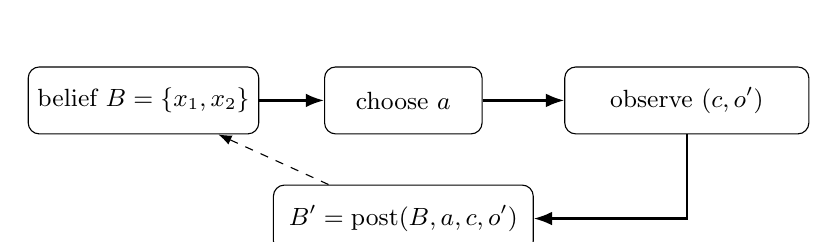
\begin{tikzpicture}[>=Latex,every node/.style={font=\small}]
\node[draw,rounded corners,minimum width=2.8cm,minimum height=.85cm] (b) at (0,0) {belief $B=\{x_1,x_2\}$};
\node[draw,rounded corners,minimum width=2cm,minimum height=.85cm] (a) at (3.3,0) {choose $a$};
\node[draw,rounded corners,minimum width=3.1cm,minimum height=.85cm] (r) at (6.9,0) {observe $(c,o')$};
\node[draw,rounded corners,minimum width=3.3cm,minimum height=.85cm] (bp) at (3.3,-1.5) {$B'=\mathrm{post}(B,a,c,o')$};
\draw[->,thick](b)--(a);\draw[->,thick](a)--(r);\draw[->,thick](r) |- (bp);
\draw[->,dashed](bp)--(b);
\end{tikzpicture}
\caption{The complete visible history becomes a finite information-set state.}
\end{figure}

\begin{theorem}[Exact finite belief-game forcing]\label{thm:belief}\hypertarget{stmt:belief}{}
For a finite partially observed certified game with publicly observed costs and target status, the minimum sure-forced settlement cost from $H$ equals the minimum forced cost in its finite perfect-information belief game:
\[
\boxed{V_M(H)=V_{\mathrm{Bel}(M)}(H).}
\]
It is therefore decidable and belongs to $\N\cup\{+\infty\}$ within the explicit contract. When finite, a finite-memory observation-based strategy and a finite worst-case bound can be extracted.
\end{theorem}\backproof{belief}

The belief game can have exponentially many information sets. Decidability is therefore not a performance claim. In particular, an unknown original program's true state space, actual hidden information, or unbounded history is not guaranteed to admit this finite representation.

\section{Evidence can strictly improve forcing without changing truth}
\begin{definition}[Observation refinement]
A finer observation $o_f:X\to O_f$ \emph{refines} a coarser observation $o_c:X\to O_c$ when $o_c=r\circ o_f$ for a fixed function $r$. Both representations use the same admitted actions, transitions, target, and charges. The refinement itself is assumed available at zero acquisition cost for this definition; any real receipt cost is charged separately.
\end{definition}

\begin{theorem}[Information-refinement dominance]\label{thm:info}\hypertarget{stmt:info}{}
For the same finite hidden-state game, if $o_f$ refines $o_c$ at zero additional charge, then
\[
 V_{(M,o_f)}(H)\ \le\ V_{(M,o_c)}(H),
\]
with the convention that every finite value is less than $+\infty$.
\end{theorem}\backproof{info}

The inequality is weak, not automatically strict. A finer receipt may reveal a fact irrelevant to the best policy. Conversely, refining a free observation is mathematically different from buying it: if a receipt costs $d$ once, the full revised path cost is $d+V_{(M,o_f)}(H)$ under the specified charges, and economic superiority needs a comparison with the admitted baseline.

\begin{example}[One bit can turn impossibility of forcing into finite settlement]\label{ex:twobit}
Let $H=\{L,R\}$, controller actions $A=\{u,v\}$, target $t$, and losing sink $\bot$. Every initial action costs $1$. At $L$, $u$ reaches $t$ and $v$ reaches $\bot$; at $R$, $v$ reaches $t$ and $u$ reaches $\bot$. The sink has a cost-zero self-loop and cannot reach $t$. Without a distinguishing receipt, the two states have the same observation; whichever initial action the controller chooses, the opponent can select the wrong hidden state. Hence $V(H)=+\infty$. If a truthful, accepted receipt says either $L$ or $R$ before the choice, the controller takes $u$ or $v$ respectively and forces $t$ at cost $1$; with an additional receipt charge $d$, total guaranteed cost becomes $d+1$. No new theorem, axiom, physical transition, or worker ability was introduced.
\end{example}

\begin{figure}[ht]
\centering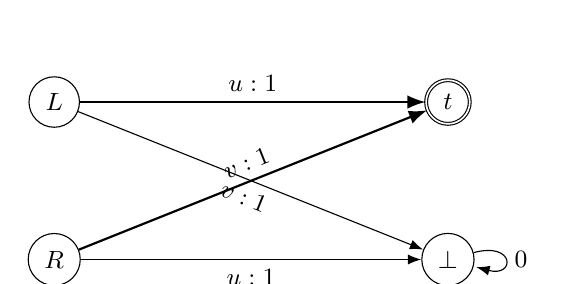
\begin{tikzpicture}[>=Latex,every node/.style={font=\small}]
\node[draw,circle] (l) at (0,1) {$L$}; \node[draw,circle] (r) at (0,-1) {$R$};
\node[draw,double,circle] (t) at (5,1) {$t$};\node[draw,circle] (s) at (5,-1) {$\bot$};
\draw[->,thick](l)--node[above]{$u:1$}(t);
\draw[->](l)--node[below,sloped]{$v:1$}(s);
\draw[->,thick](r)--node[above,sloped]{$v:1$}(t);
\draw[->](r)--node[below]{$u:1$}(s);
\draw[->] (s) edge[loop right] node{$0$}(s);
\end{tikzpicture}
\caption{Same action graph, different information: a truthful receipt selects the safe branch.}
\end{figure}

\section{A minimum receipt theorem}
We now remove the incidental dynamics of the preceding example and isolate a mathematical measure of the evidence needed for a \emph{single} certified decision. Fix a finite nonempty hidden-state set $H$, action set $A$, common budget threshold $b\in\N$, and a complete transition table. A one-step action is accepted only when all of its possible charged successors meet the stipulated target and cost requirements.

\begin{definition}[Uniformly winning action domains]
For each action $a\in A$, define
\[
 S_a(b)=\big\{x\in H: a\text{ is legal at }x\text{ and every }(c,y)\in\delta(x,a)\text{ has }c\le b,\ y\in T\big\}.
\]
A $k$-symbol \emph{truthful receipt scheme} is a function $r:H\to\{1,\ldots,k\}$ together with one action $a_j$ for each used symbol $j$, such that $r(x)=j$ implies $x\in S_{a_j}(b)$. The scheme may be used only if the contract actually authorizes producing and checking such a truthful receipt. Here we measure message alphabet size, not physical acquisition cost.
\end{definition}

\begin{theorem}[Minimum receipt alphabet equals minimum action cover; candidate-original relative to W0--W2]\label{thm:cover}\hypertarget{stmt:cover}{}
Let $k_*(b)$ be the smallest number of receipt symbols permitting a guaranteed one-step settlement under the preceding definition. Let $\mathcal S_b=\{S_a(b):a\in A\}$. Then
\[
\boxed{\quad k_*(b)=\min\Big\{|C|:C\subseteq A,\ \bigcup_{a\in C}S_a(b)=H\Big\}.\quad}
\]
If no such cover exists, both sides are $+\infty$. If $k_*(b)<\infty$, a fixed-length binary encoding of an ideal truthful receipt needs exactly $\lceil\log_2 k_*(b)\rceil$ bits. The finite optimum and an explicit scheme can be found by enumerating action subsets.
\end{theorem}\backproof{cover}

This result turns a question about epistemic accessibility into a combinatorial invariant of an explicitly certified action table. It is deliberately not a theorem that a useful receipt can be \emph{discovered or obtained} for free. A true statement about which action works can be costly or impossible to certify within the authorized resources.

\begin{corollary}[More generous cost thresholds need no more messages]\label{cor:monob}\hypertarget{stmt:monob}{}
If $b'\ge b$, then $k_*(b')\le k_*(b)$, with $+\infty$ allowed. This is monotonicity of the ideal information requirement, not a statement of monotone practical implementation cost.
\end{corollary}\backproof{monob}

\begin{proposition}[Pairwise action compatibility does not imply a common action]\label{prop:pair}\hypertarget{stmt:pair}{}
There exist three hidden states such that each pair admits at least one common uniformly winning action, yet no one action works for all three. Consequently, pairwise conflict checks alone can understate $k_*(b)$.
\end{proposition}\backproof{pair}

\begin{example}[Three-way evidence obligation]\label{ex:triad}
Take $H=\{1,2,3\}$ and three actions $a,b,c$ with successful-state sets
\[
 S_a=\{1,3\},\qquad S_b=\{1,2\},\qquad S_c=\{2,3\}.
\]
Every two states share some one-step successful action, but $S_a\cap S_b\cap S_c$ is irrelevant: the decisive fact is that \emph{no single} $S_a$ covers all three. Any two of the actions cover $H$, hence $k_*=2$. A binary receipt distinguishes the cell requiring one action from the complementary cell requiring the other. The construction can be realized as a finite deterministic transition table in which a successful action reaches $t$ and every unsuccessful action reaches the absorbing sink.
\end{example}

\begin{figure}[ht]
\centering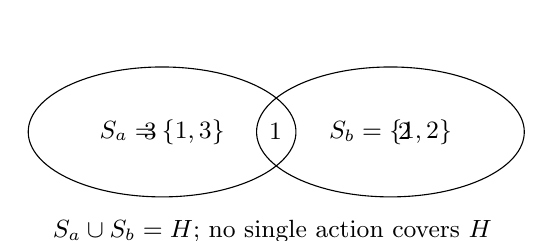
\begin{tikzpicture}[>=Latex,every node/.style={font=\small}]
\node[draw,ellipse,minimum width=3.4cm,minimum height=1.65cm] at (0.9,0) {$S_a=\{1,3\}$};
\node[draw,ellipse,minimum width=3.4cm,minimum height=1.65cm] at (3.8,0) {$S_b=\{1,2\}$};
\node at (2.34,0) {$1$};\node at (0.75,0) {$3$};\node at (3.98,0) {$2$};
\node[below=1cm] at (2.3,0) {$S_a\cup S_b=H$; no single action covers $H$};
\end{tikzpicture}
\caption{Pairwise compatibility need not produce a common global settlement action.}
\end{figure}

\section{Certification and the price of the receipt}
Under a frozen contract, three distinct objects must be checked. First, the \emph{transition certificate} supports the assertion that each $S_a(b)$ has been computed from an exhaustive admissible transition table. Second, a \emph{receipt-fidelity certificate} shows that the observed symbol is truthful for the actual hidden state. Third, an \emph{economic certificate} includes the cost of producing, validating, communicating, and retaining that receipt, as well as the cost of the selected action, failures, and reuse.

\begin{proposition}[Receipt cover is a conditional sufficiency certificate]\label{prop:conditional}\hypertarget{stmt:conditional}{}
A finite accepted transition table and a checked action cover certify the existence of an abstract one-step receipt policy \emph{if truthful receipts are available}. They do not certify that a proposed machine can produce a truthful receipt, that the receipt is independent of its controller's untrusted assertion, or that acquiring it lowers total expenditure.
\end{proposition}\backproof{conditional}

For $N$ repetitions, suppose a verifier certifies per-episode old lower bound $p$, new upper bound $q$, and complete acquisition and deployment upper bound $B$. Then $N(p-q)>B$ gives a strict net gain against the frozen old policy (W0 V.6; W1 and W2). If the old forced cost was $+\infty$, a new finite forced path is an improvement in \emph{guarantee} but should not automatically be reported as an economic savings of ``infinite dollars'': its meaning depends on the contract's accounting and feasibility obligations.

\section{What the new theory rules out}
An absent receipt does not prove that the underlying mathematical question is independent or physically impossible. It may mean only that the controller cannot distinguish two live states under the currently permitted observations. Likewise, a receipt scheme using $k$ abstract symbols does not provide a deployed sensing instrument, a proof-generating ATP, or an oracle for unknown semantic program equivalence. If an allowed action changes hidden information or the checker state during a sequence of steps, the one-step cover theorem no longer solves the multi-step problem; the complete belief game is required.

The finite model separates four boundaries: logical preservation (W0), safe behavior under all admitted branches (W1), future-sufficient representation (W2), and evidence sufficiency for a partially informed controller (W3). The new mathematical identity is not a new name for the same revision theorem: it is the quantitative structure of \emph{which distinctions the controller must learn before it can guarantee an outcome}.

\section{Research ledger and originality tests}
\small
\begin{longtable}{p{0.19\linewidth}p{0.37\linewidth}p{0.31\linewidth}}
\toprule Classification & Development & Closest antecedent and obligation \\\midrule\endhead
Inherited & Certificate-gated revision and epistemic evidence distinction & W0 III--IV; no phenomenology claim \\
Inherited & Exact finite forcing; certified state compression & W0 V--VI; W1--W2 finite game quotient \\
Derived / candidate-original relative to lineage & Theorem~\ref{thm:belief}: cost-visible partial-observation belief-game translation & New formal question; proof in PROOFS, external-priority unknown \\
Derived & Theorem~\ref{thm:info}: finer free observation cannot worsen a forced outcome & Direct policy simulation \\
Candidate-original relative to W0--W2 & Theorem~\ref{thm:cover}: minimum one-step receipt symbols equal minimum action cover & Explicit proof; not asserted to be novel in outside literature \\
Counterexample & Two-state forced-cost jump and three-state pairwise failure & Finite models; no installed experiment \\
Unresolved & Cost and feasibility of real receipt discovery, partial information in unbounded ATPs & Requires separately checked fidelity and resource contract \\
\bottomrule\end{longtable}
\normalsize

The five originality tests from the research prompt have the following restricted findings: (1) the receipt-cover problem is meaningful without reading W0--W2; (2) the cover theorem provides a substantive finite derivation not found in the supplied manuscript; (3) the combinatorial object was motivated by the hidden-state obstruction, not by renaming an older theorem; (4) paper proofs and explicit finite counterexamples are supplied, but no independent kernel check; (5) every statement above is separated by source and status. External originality and implementation validity remain unresolved.


\section{Comparison of three Level-3 candidates}
The Level-3 investigation tested three substantive directions. \emph{A3 (structural)} continued W2's strong state-quotient theory into larger labeled games; it was mathematically coherent but did not produce a sufficiently different central question. \emph{B3 (conceptual)} replaced equivalence of hidden states by the minimum evidence needed to choose a uniformly successful action; this yielded the receipt-cover theorem. \emph{C3 (emergent synthesis)} connected hidden evidence with W1's adversarial cost semantics through a finite belief-game construction. The completed manuscript uses B3 as its new mathematical identity and C3 as its multi-step foundation, while retaining A3's reminder that no state or proof obligation may be erased without a fidelity argument.

The originality claim is deliberately ancestry-relative. The finite belief-state method and the set-cover characterization may have antecedents in the mathematical literature, which the prompt prohibits consulting here. No external priority is asserted. The substantive separation from W0--W2 is the new quantity $k_*(b)$: the least alphabet size of a truthful receipt that suffices for a guaranteed one-step action in a frozen hidden-state contract.

\section{PROOFS}
\hypertarget{proof:belief}{}\subsection*{Theorem \ref{thm:belief}: belief-game equivalence} \backstatement{belief}
Every observation-based policy in $M$ induces a policy on reachable beliefs, since the belief after a visible finite history is computed recursively from that history. Conversely, every belief-game policy is an observation-based policy: the controller knows the same publicly visible actions, costs, and observations needed to update its belief. A finite sequence of belief-game replies is feasible exactly when there exists an original run from $H$ producing that visible sequence: induction on the number of observations establishes this using the definition of $\mathrm{post}$. Thus each finite cost and reachability prefix admitted in one model corresponds to a feasible prefix in the other.

For infinite sequences the issue is whether the belief adversary could switch among incompatible hidden paths. Fix an infinite feasible visible sequence. For each length, the tree of original hidden-state prefixes realizing its first that many records is nonempty and finitely branching, since $X$ and each $\delta(x,a)$ are finite. K\"onig's finite-branching argument yields an infinite compatible hidden run. Thus an infinite avoiding visible play is feasible in the original system, not an artifact of the belief construction. Because membership in $T$ is visible and $T$ is absorbing, a belief is contained in $T$ exactly when all runs compatible with that public record have reached the target. The reachability and worst-case accumulated cost outcomes therefore match for every fixed observation-based controller policy. Taking its infimum yields equality of forced values. The belief game is finite (its positions are nonempty subsets of a finite $X$), so finite-game reachability and budget expansion decide the value and extract a rank-based finite-memory policy. Zero-cost infinite loops are correctly losing. This proof requires the stated target observability and public cost records.

\hypertarget{proof:info}{}\subsection*{Theorem \ref{thm:info}: observation dominance} \backstatement{info}
Given a fine-observation history, apply $r$ pointwise to recover the coarse-observation history and then execute the controller policy prescribed by the coarse system. This is a legal fine-observation policy with exactly the same actions, admissible adversarial continuations, and costs. Therefore every bound achievable with coarse information is achievable with fine information. Taking the infimum proves the inequality, including the case of $+\infty$.

\hypertarget{proof:cover}{}\subsection*{Theorem \ref{thm:cover}: minimum action cover} \backstatement{cover}
Suppose a truthful scheme uses $k$ symbols. Each nonempty receipt cell $H_j=\{x:r(x)=j\}$ is contained in $S_{a_j}(b)$ by the definition of a successful scheme. The selected action domains therefore cover $H$ using at most $k$ actions. Hence the minimum action-cover number is at most $k$.

Conversely, suppose $C\subseteq A$ is a smallest family with $\cup_{a\in C}S_a(b)=H$. For every $x\in H$, choose one covering action $a(x)\in C$ with $x\in S_{a(x)}(b)$. Let the receipt identify $a(x)$ and have the controller use that action. Each cell consists only of states on which its action is uniformly winning with charge at most $b$. Thus a truthful scheme exists using at most $|C|$ symbols, so $k_*\le |C|$. The two inequalities give equality. If some state belongs to no $S_a(b)$, no cover and no valid scheme exists. Finally, $k$ distinct symbols require at least $\lceil\log_2 k\rceil$ fixed-length bits and can be encoded using exactly that many; this is an encoding count, not a physical implementation theorem. Finite exhaustive enumeration over action subsets computes $k_*$ and a witnessing receipt assignment.

\hypertarget{proof:monob}{}\subsection*{Corollary \ref{cor:monob}: threshold monotonicity} \backstatement{monob}
For $b'\ge b$, every action-success set $S_a(b)$ is a subset of $S_a(b')$, since the only changed requirement is a weaker upper bound on visible cost. Every cover valid at $b$ remains a cover at $b'$, so the minimum number of domains needed cannot increase.

\hypertarget{proof:pair}{}\subsection*{Proposition \ref{prop:pair}: pairwise failure} \backstatement{pair}
Use the three success domains in Example~\ref{ex:triad}. States $1,2$ share action $b$; states $1,3$ share $a$; states $2,3$ share $c$. Yet none of $a,b,c$ covers $\{1,2,3\}$, so a one-symbol receipt is impossible. Any two domains cover all states, so by Theorem~\ref{thm:cover} exactly two receipt symbols are sufficient. This establishes the claimed failure of a pairwise-only test.

\hypertarget{proof:conditional}{}\subsection*{Proposition \ref{prop:conditional}: conditional sufficiency} \backstatement{conditional}
The covering assignment provides an abstract function from the actual hidden state to a symbol and a successful action for each symbol. It is a statement of existence within the state/action table. The premises make no claim about the computability, physical accessibility, independent checkability, or acquisition cost of the map from a real hidden state to its symbol. No conclusion about these additional properties follows without adding and verifying the relevant premises; in particular, a self-declared receipt could be false. This is a logical separation, not a claim that implementation is impossible.
\section*{Source and verification notes}
\addcontentsline{toc}{section}{Source and verification notes}
The sole mathematical research input for this development was the user-supplied 68-page manuscript \emph{Certified Self-Improving Mathematical Discovery: Parts II--VI}, strengthened ATLAS v2 edition dated 15 November 2026 (here called W0). Section references to W0 are internal source attributions, not claims that its original external bibliography has been independently consulted. W0 itself identifies ChatGPT (OpenAI) as its editorial author and Brian Tenneson as research director. W0 remains unaltered. The new research articles are AI-assisted drafts under Brian Tenneson's research direction; their mathematical novelty has only been compared with the supplied ancestry, not with the wider literature.

All proofs in this manuscript are human-readable paper arguments, reviewed internally but \emph{not} independently formally checked. Any finite checker mentioned is part of the stated mathematical model. No deployed FORGE-6/CAMI machine, hardware benchmark, new experiment, or independent proof-kernel receipt is represented as having occurred. Claims about external priority, unrestricted computation, and improvement of any real implementation remain open.

\section*{AI disclaimer and attribution}\addcontentsline{toc}{section}{AI disclaimer and attribution}
This research exposition and its diagrams were drafted with AI assistance, with research direction attributed to Brian Tenneson. AI assistance does not substitute for independent proof checking or external mathematical peer review. Historical authorship of W0 is preserved in the source and verification notes. The conditional theorems here concern explicit mathematical contracts, not autonomous self-modification of ChatGPT or proof of machine consciousness.
\end{document}
